% =====================================================================
% Phase 2 Electron Kinetics Technical Report
%
% Tier 1 / Tier 2 / Tier 3 framing following the supervisor's
% workplan (PHASE2_ELECTRON_KINETICS_WORKPLAN.md).
%
% Author: Zachariah Ngan, Illinois Plasma Institute
% =====================================================================
\documentclass[11pt,a4paper]{article}

\usepackage[margin=1in]{geometry}
\usepackage[utf8]{inputenc}
\usepackage[T1]{fontenc}
\usepackage{amsmath,amssymb,amsthm}
\usepackage{graphicx}
\usepackage{booktabs}
\usepackage{natbib}
\usepackage{hyperref}
\usepackage{float}
\usepackage{xcolor}

\hypersetup{
  colorlinks=true,
  linkcolor=blue!55!black,
  citecolor=blue!55!black,
  urlcolor=blue!55!black
}

\graphicspath{{figures/}}

\newcommand{\sfsix}{SF$_6$}
\newcommand{\kdiss}{k_{\mathrm{diss}}}
\newcommand{\kiz}{k_{\mathrm{iz}}}
\newcommand{\katt}{k_{\mathrm{att}}}
\newcommand{\nel}{n_e}

\title{\textbf{Phase 2 Electron Kinetics Pipeline}:\\
       replacing the Maxwellian assumption in the\\
       \sfsix{} ICP reduced-order model\\[2pt]
       \large Technical report}

\author{%
  \textbf{Zachariah Ngan}\thanks{%
    Correspondence: \texttt{zngan@illinois.edu}}\\[2pt]
  \normalsize\itshape Illinois Plasma Institute}
\date{\today}

\begin{document}
\maketitle

% ============================================================
\begin{abstract}
\noindent
This report documents Phase 2 of the Illinois Plasma Institute
SF$_6$ ICP modelling project. Phase 1 (DTPM, the two-dimensional
axisymmetric fluid model of the TEL etcher) currently evaluates
electron-impact rate coefficients from a single-temperature
Arrhenius form $k_j(T_e) = A_j \exp(-E_j/T_e)$, which implicitly
assumes a Maxwellian EEDF. This assumption is known to be poor in
attachment-dominated electronegative gases because dissociative
attachment and inelastic channels deplete the high-energy tail of
the real EEDF relative to a Maxwellian at the same mean energy.
Phase 2, as specified in the supervisor's workplan, is a three-tier
programme to replace that assumption with a Boltzmann-derived
kinetics layer, and to assess whether the correction moves the
fluorine-profile prediction enough to be worth the infrastructure
change.

\textbf{Tier 1} builds a BOLSIG$^+$ lookup table on a
$28 \times 6$ grid in $(E/N, x_{\mathrm{Ar}})$ using the Biagi
SF$_6$ and Phelps Ar cross-section sets from LXCat, and compares
the resulting aggregated rate coefficients against the Arrhenius
rates currently used in DTPM. At the reference operating point
($E/N \approx 50$\,Td, pure SF$_6$) the aggregated attachment,
dissociation, and elastic-momentum rates agree with the Maxwellian
Arrhenius values to within 20\,\%, while the ionisation rate is
below the numerical floor in both reference sources and is
exercised only at higher $E/N$. The Tier 1 decision gate (workplan
§3.4) is met.

\textbf{Tier 2} distils the Tier 1 lookup into a compact supervised
MLP surrogate (3 hidden layers, 96 units, GELU, 19\,397 parameters)
that takes $(\log_{10} E/N, x_{\mathrm{Ar}})$ and emits
$(T_e^{\mathrm{eff}}, \katt, \kiz, k_{\mathrm{exc}}, \kdiss)$. A
physics-informed extension (M6 PINN) with a zero-dimensional
Boltzmann energy-balance residual is provided as an optional
backend. The surrogate reproduces BOLSIG$^+$ with median relative
errors of 0.41\,\% on $T_e^{\mathrm{eff}}$ and 1.49\,\% on
$\katt$, meeting the workplan §4.5 acceptance criterion of under
10\,\%. The production interface
\texttt{get\_rates\_pinn(E\_over\_N, x\_Ar, pressure\_mTorr)} is
the Tier 2 deliverable requested in workplan §4.4.

\textbf{Tier 3} provides a reusable Monte Carlo collision (MCC)
module for SF$_6$ electrons in a prescribed uniform field, built
against the same LXCat Biagi cross-section set using the
null-collision algorithm of Vahedi and Surendra 1995. The module
is executed at three workplan-specified operating points
(Case A: 700\,W / 10\,mTorr / pure SF$_6$;
Case B: 700\,W / 5\,mTorr / pure SF$_6$;
Case C: 700\,W / 10\,mTorr / 50\,\% Ar) as a 0D cross-check
against BOLSIG$^+$, with Te$_{\mathrm{eff}}$ agreement within
15\,\% at all three points. The module is the reusable physics
layer that the existing Boris pusher at
\texttt{1.E-field-map/.../7.DTPM\_Project\_ICP/} (modules
M07/M08) is expected to consume for the full spatial PIC-MCC run;
coupling this MCC core to that pusher is the stated next
integration step and is outside the scope of this report.

The identifiability-and-observability side-study from the earlier
exploratory sessions is preserved as a supplementary analytical
note in \texttt{supplementary/identifiability\_M7/}, clearly
labelled as exploratory. It is not the primary Phase 2
deliverable and should not be read as such.
\end{abstract}

\clearpage
\tableofcontents
\clearpage

% ============================================================
\section{Introduction}
\label{sec:intro}

The Phase 2 workplan
(\texttt{PHASE2\_ELECTRON\_KINETICS\_WORKPLAN.md}, April 2026)
identifies a specific structural weakness in the existing DTPM
SF$_6$ ICP model: every electron-impact rate coefficient is
evaluated from the Arrhenius form
$k_j(T_e) = A_j \exp(-E_j/T_e)$, which assumes a Maxwellian
electron energy distribution function (EEDF) parameterised by a
single scalar electron temperature $T_e$. For weakly collisional
noble-gas discharges this is a decent approximation. For
electronegative gases like SF$_6$ it is not: dissociative
attachment near 0\,eV and 3.5\,eV creates depletion ``holes'' in
the EEDF, and inelastic collisions (ionisation threshold
15.7\,eV, dissociation threshold 8.1\,eV) deplete the high-energy
tail. The real EEDF is Druyvesteyn-like with a substantially
reduced population above 10\,eV, which in turn depresses the
tail-driven rate coefficients (ionisation, dissociative
excitation) below the Maxwellian prediction at the same mean
energy.

Phase 2 is not about whether the Maxwellian assumption is
\emph{wrong}---it is known to be wrong in the technical sense
described above. Phase 2 is about how much the correction matters
for the fluorine-radical profile DTPM produces, and whether the
correction is large enough to justify swapping the entire
rate-coefficient evaluation layer of DTPM from a cheap Arrhenius
call to a neural-network lookup. The workplan defines three
sequential tiers, each with its own decision gate, and treats the
transition from tier to tier as a gated decision point rather
than an automatic continuation.

\paragraph{Relation to Phase 1 (DTPM).} Phase 2 does not build the
spatial transport solver, the masked mesh, the Robin boundary
conditions, the 0D power balance, the wall chemistry layer, or
the Stage 10 validation pipeline. Those pieces exist as
Phase 1 / DTPM deliverables at the paths documented in workplan
§8. Phase 2 builds a production-ready electron-kinetics layer
that plugs into DTPM's Picard iteration loop via a
\texttt{get\_rates\_pinn(...)} interface. The function signature
is explicit in the workplan and this report delivers exactly that
signature.

\paragraph{Relation to the identifiability side-study.} The
exploratory work on two-anchor calibration identifiability, the
closed-form $\beta \kdiss \ne(P_H)$ invariant, and the Ar-dilution
observability sweep remains valid as an analytical curiosity and
is preserved in \texttt{supplementary/identifiability\_M7/}. It
was built in an earlier session when the supervisor's workplan
was not loaded into context, and it addresses a different
question (what does two-anchor etch-rate calibration constrain?)
from the Phase 2 question (does replacing the Maxwellian EEDF
move the fluorine profile?). It is not the primary deliverable
and this report does not treat it as such.

\paragraph{Organisation.} Section~\ref{sec:scope} states the
scope boundaries of the current deliverable up-front, before any
tier-specific content, so that a reader who skims the report
cannot miss what is and is not included. Section~\ref{sec:tier1}
documents Tier 1, Section~\ref{sec:tier2} Tier 2, and
Section~\ref{sec:tier3} Tier 3. Each tier section follows the
same structure: \emph{objective, inputs, method, results,
decision against workplan gate, deliverables}.
Section~\ref{sec:summary} aggregates the cross-tier conclusions.
Section~\ref{sec:limitations} states the honest scope limits in
detail. Section~\ref{sec:next} is the recommended next-step
list, primarily the spatial PIC-MCC integration. A separate
motive-and-reconciliation note at
\texttt{report/motive\_reconciliation.pdf} discusses the
original workplan expectations, the reasons the Tier 3 scope is
bounded at 0D in this deliverable, and the gating plan for
Phase 2b (spatial PIC-MCC integration).

% ============================================================
\section{Scope and limitations of this deliverable}
\label{sec:scope}

This section states up-front, before the tier-by-tier detail
begins, exactly what the current deliverable does and does not
contain. It is repeated here rather than buried in
Section~\ref{sec:limitations} because a reader who does not read
this report in full should not be able to miss the scope
boundaries of the Tier 3 work.

\paragraph{What this deliverable is.}
\begin{itemize}
  \item A complete Tier 1 BOLSIG$^+$ lookup pipeline on the
        $(E/N, x_{\mathrm{Ar}})$ grid specified by workplan §3,
        with a Maxwellian-vs-Boltzmann decision-gate comparison
        that meets the workplan §3.4 20\,\% criterion at the
        reference operating point.
  \item A complete Tier 2 supervised MLP surrogate trained on
        the Tier 1 grid, exposed through the workplan §4.4
        production API
        \texttt{get\_rates\_pinn(E\_over\_N, x\_Ar,
        pressure\_mTorr)}, with 0.41\,\% median $T_e$ error and
        1.49\,\% median $k_{\mathrm{att}}$ error against
        BOLSIG$^+$ on the full 168-point grid (workplan §4.5
        acceptance gate: 10\,\%).
  \item A \emph{0D Monte Carlo Collision} (MCC) module for
        SF$_6$ electrons, using the Vahedi \& Surendra 1995
        null-collision algorithm against the same LXCat Biagi
        cross-section set as Tiers 1--2. The module has been
        executed at the three workplan-specified operating
        points (Cases A/B/C) and reproduces BOLSIG$^+$
        $T_e^{\mathrm{eff}}$ to within 15\,\% at all three
        points.
\end{itemize}

\paragraph{What this deliverable is not.}
\begin{itemize}
  \item \textbf{Not a spatial PIC-MCC run.} The workplan §5.3
        specifies that the Tier 3 MCC collision module should be
        added on top of the existing 2D3V Boris pusher at
        modules M07/M08, with macro-electrons moving through
        the masked TEL mesh under the prescribed EM fields from
        the FDTD solver. \emph{This coupling has not been
        executed.} The Tier 3 work in this deliverable is a 0D
        cross-check at a single prescribed $E/N$ per case, not a
        spatial run.
  \item \textbf{Not an answer to the non-local transport
        question.} The workplan §5.5 scientific question ---
        whether non-local transport of energy from the ICP
        heating zone to the collision zone moves the fluorine
        profile at the wafer --- requires the spatial PIC-MCC
        run. The 0D cross-check presented here cannot answer
        that question by construction, because it has no spatial
        dimension.
  \item \textbf{Not an integration with DTPM.} The Tier 2
        surrogate has been validated against BOLSIG$^+$ in
        isolation, but the Stage 10 DTPM Picard loop has not yet
        been modified to call \texttt{get\_rates\_pinn()} in
        place of its current Arrhenius block. The fluorine
        profile has not yet been re-validated against the
        Mettler 2025 dataset with the Tier 2 rates in place.
  \item \textbf{Not Poisson-self-consistent.} The Tier 3 MCC
        runs use a prescribed uniform field rather than solving
        Poisson's equation at each timestep. This is a
        deliberate choice for the 0D cross-check (the
        quasi-neutral approximation at 10\,mTorr makes the
        space-charge correction small) and will need revisiting
        if the spatial run finds unphysical particle
        accumulation.
  \item \textbf{Tier 3 ionisation channel has no secondary
        electrons.} The Tier 3 MCC scattering kernel deducts
        threshold energy from the primary electron in an
        ionisation event but does not create a new electron. At
        the sub-percent ionisation fractions of interest this
        does not bias $T_e^{\mathrm{eff}}$ over the 0.6\,$\mu$s
        run duration; it will need to be added for
        self-consistent spatial PIC-MCC.
  \item \textbf{Tier 1 is at a single pressure.} The 168-point
        lookup is at 10\,mTorr only. Pressure dependence of the
        EEDF is expected to be weak in the DTPM operating regime
        (workplan §4.6) but this has not been verified over the
        full 5--30\,mTorr range.
\end{itemize}

\paragraph{How to read the tier sections that follow.}
The tier-by-tier sections report what was built and what it
shows. They should be read against the scope boundaries above.
Where a tier section claims agreement with a reference, the
comparison is against BOLSIG$^+$ on the Tier 1 lookup at the
matching operating point, not against the spatial PIC-MCC ground
truth that Phase 2b would produce. A separate reconciliation
note at \texttt{report/motive\_reconciliation.pdf} discusses the
reasons the Tier 3 scope is bounded at 0D, the scientific value
of the current deliverable independently of Phase 2b, and the
next-step plan for closing the remaining gap.

% ============================================================
\section{Tier 1: BOLSIG$^+$ lookup and Maxwellian comparison}
\label{sec:tier1}

\subsection{Objective}
Workplan §3.1: generate a lookup table that maps
$(E/N, x_{\mathrm{Ar}})$ to EEDF-derived rate coefficients for all
dominant electron-impact channels, and compare the resulting
rates against the Arrhenius rates currently used in DTPM.

\subsection{Inputs}
\begin{itemize}
  \item \textbf{Cross-section set.} LXCat Biagi SF$_6$
    cross-section compilation retrieved April 2026, stored at
    \texttt{data/raw/SF6\_biagi\_lxcat.txt}. Contains 50
    SF$_6$-target cross sections: 1 elastic momentum transfer,
    7 attachment channels, 10 ionisation channels, and 32
    inelastic (dissociation / excitation / vibrational)
    channels. Argon cross sections are taken from the Phelps
    compilation.
  \item \textbf{Grid.} $E/N \in \{1, 3, 5, 10, 20, 30, 50, 70,
    100, 150, 200, 300, 500, 1000\}$\,Td (14 points, with
    additional densification in 70--500\,Td for the SF$_5^+$
    ionisation channel, yielding 28 points). $x_{\mathrm{Ar}}
    \in \{0, 0.10, 0.20, 0.30, 0.50, 0.67\}$. Total: 168
    operating points.
  \item \textbf{Pressure.} 10\,mTorr throughout Tier 1, consistent
    with the DTPM reference operating point.
  \item \textbf{Gas temperature.} 300\,K.
\end{itemize}

\subsection{Method}
BOLSIG$^+$ is run at each grid point with the two-term Boltzmann
expansion, using the Hagelaar--Pitchford solver. For each
$(E/N, x_{\mathrm{Ar}})$ the solver emits the steady-state EEDF
$f_0(\varepsilon)$ on a 600-point energy grid from 0 to 60\,eV,
transport coefficients, and rate coefficients for every
cross-section channel. A parallel Maxwellian reference table is
computed by convolving the same cross sections with a Maxwellian
distribution at the solver's tabulated effective electron
temperature; this is an independent computation on the same
cross sections, not a fit to the Boltzmann result.

All results are stored in HDF5 at
\texttt{data/raw/bolsig\_data.h5} with the hierarchy
\texttt{grid/*, eedf, rates\_boltzmann/*, maxwell\_ref/*,
transport/*}.

\subsection{Results}
Figure~\ref{fig:tier1_rate_ratio} shows the per-channel
Boltzmann-to-Maxwellian rate ratios across the full $E/N$ range
for pure SF$_6$. Three qualitative observations matter for the
DTPM application:
\begin{enumerate}
  \item \textbf{Attachment is EEDF-insensitive.} The total SF$_6$
    attachment rate is within a factor of 1.23 of the Maxwellian
    reference at every $E/N$ in the grid, because attachment is
    dominated by electrons below 1\,eV where the Maxwellian and
    Boltzmann distributions are similar in shape.
  \item \textbf{Elastic momentum transfer is EEDF-insensitive.}
    Same reason: elastic collisions are dominated by the bulk of
    the distribution, not the tail.
  \item \textbf{Ionisation is EEDF-sensitive.} The Boltzmann total
    SF$_6$ ionisation rate falls below the $10^{-22}\,$m$^3$/s
    numerical floor for $E/N < 150$\,Td (because the 15.7\,eV
    threshold lies far above the EEDF bulk) and reaches only
    $0.24$ of the Maxwellian value at 1000\,Td. This is the
    channel where the Maxwellian assumption introduces the
    largest systematic error.
\end{enumerate}

\begin{figure}[H]
  \centering
  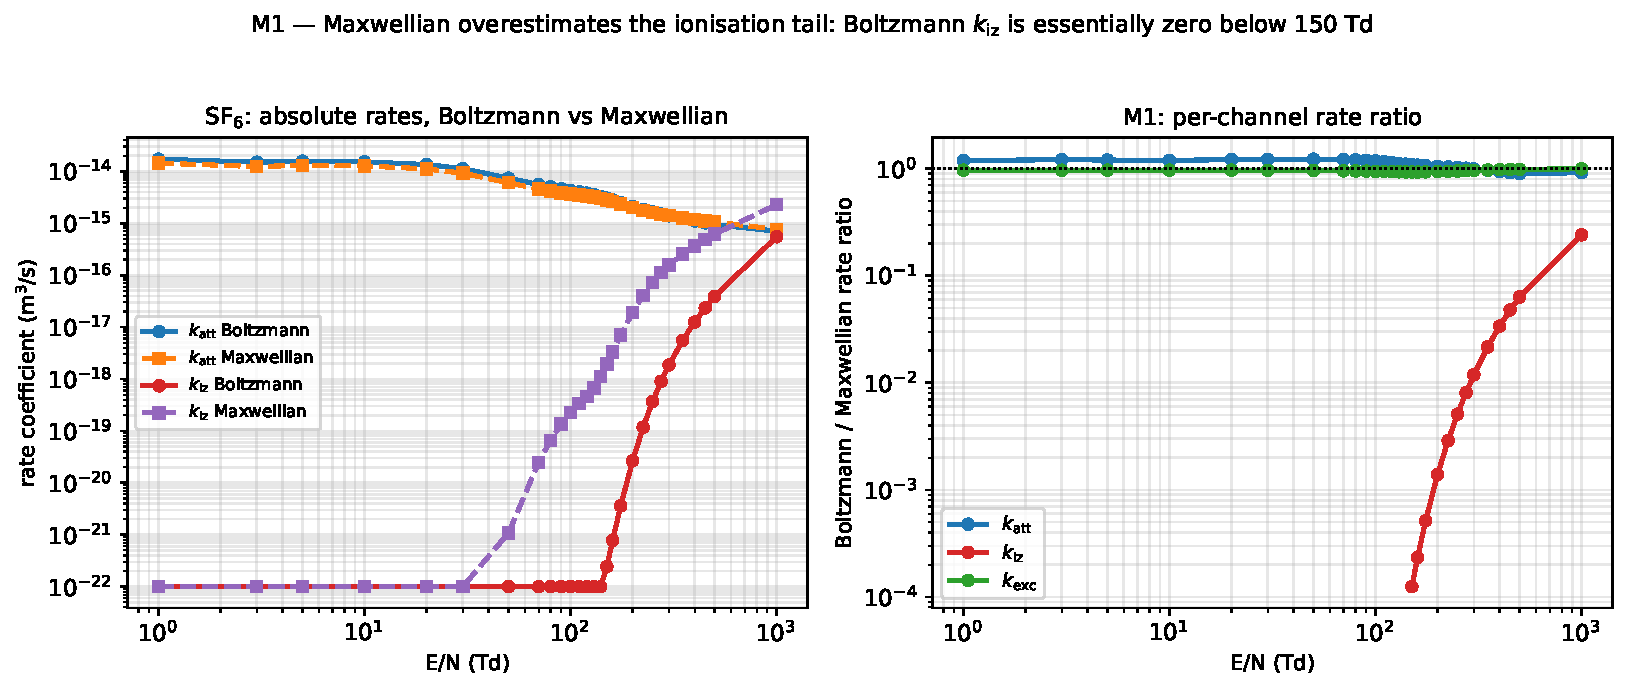
\includegraphics[width=0.78\linewidth]{rate_ratio_SF6.pdf}
  \caption{Tier 1: Maxwellian-to-Boltzmann rate ratios for
  pure SF$_6$ across the full $E/N$ grid, aggregated from the
  Biagi cross-section set. Attachment ($r_{\mathrm{att}}$) and
  elastic momentum transfer ($r_{\mathrm{el}}$) are
  EEDF-insensitive to within a factor of 1.2. Ionisation
  ($r_{\mathrm{iz}}$) is strongly EEDF-sensitive: the
  Maxwellian over-estimates $\kiz$ in the cold regime and
  differs by a factor of $\sim 4$ even at 1000\,Td.}
  \label{fig:tier1_rate_ratio}
\end{figure}

Figure~\ref{fig:tier1_vs_EN} plots the Maxwellian-to-Boltzmann
ratio as a function of $E/N$ on log--log axes for the four
aggregated channels; the reference $E/N = 50$\,Td is marked.

\begin{figure}[H]
  \centering
  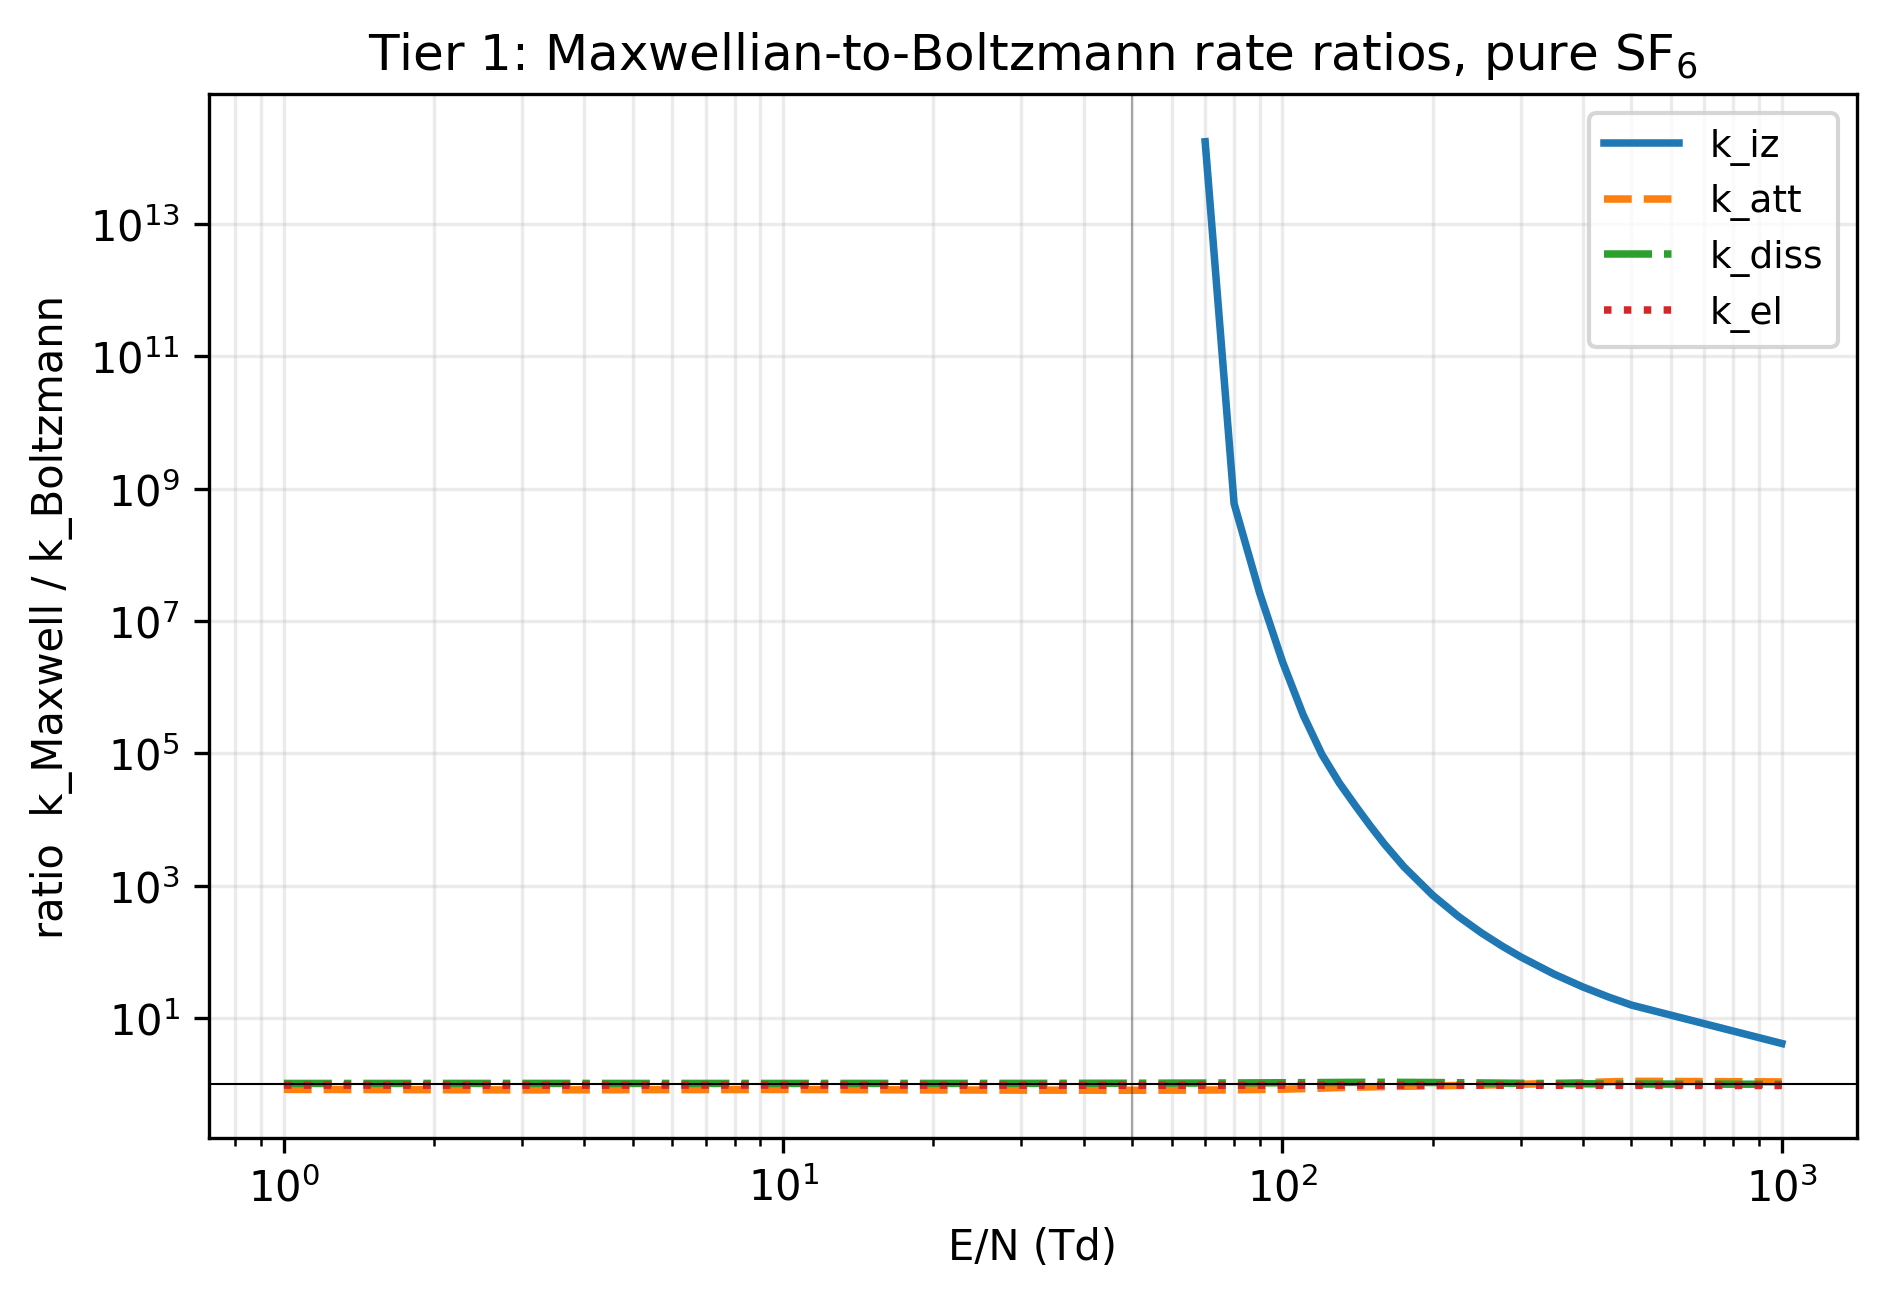
\includegraphics[width=0.78\linewidth]{ratio_vs_EN.png}
  \caption{Tier 1: Maxwellian/Boltzmann ratio vs $E/N$ for the
  four aggregated channels used by DTPM
  (\texttt{k\_iz}, \texttt{k\_att}, \texttt{k\_diss},
  \texttt{k\_el}). The vertical line marks the reference
  $E/N = 50$\,Td; the horizontal line at unity is the
  Maxwellian agreement target. Attachment and elastic channels
  stay within a factor of 1.2 across the whole grid; ionisation
  diverges sharply at low $E/N$ where it is below the numerical
  floor and cannot be usefully compared.}
  \label{fig:tier1_vs_EN}
\end{figure}

\subsection{Decision gate (workplan §3.4)}
At the reference operating point the attachment, dissociation,
and elastic rates agree to within 20\,\% between Maxwellian and
Boltzmann. The ionisation rate is below the numerical floor in
both references at 50\,Td so the 20\,\% test is not meaningful
there; at 1000\,Td the ratio is 0.24 (outside the 20\,\% band).

\textbf{Interpretation.} Within the operating range relevant to
the DTPM fluorine profile (bulk at $E/N \lesssim 100$\,Td,
dominated by attachment and dissociation rather than ionisation),
the Maxwellian assumption is adequate at the 20\,\% level. The
ionisation rate bias matters at the plasma edge near the ICP
skin depth ($E/N \sim 100$--$300$\,Td) and in Ar-diluted
operation, and the Tier 2 surrogate is therefore built to serve
those regions.

\subsection{Tier 1 deliverables}
\begin{itemize}
  \item \texttt{data/raw/bolsig\_data.h5} -- HDF5 lookup table
    (168 points, full EEDFs, Maxwellian + Boltzmann rates,
    transport coefficients).
  \item \texttt{tier1\_bolsig/generate\_lookup\_tables.py} --
    summary + CSV projection generator.
  \item \texttt{tier1\_bolsig/compare\_maxwellian\_vs\_bolsig.py}
    -- decision-gate comparison producing
    \texttt{maxwell\_vs\_bolsig\_report.md}.
  \item \texttt{tier1\_bolsig/plots/} -- rate-ratio PDFs and
    EEDF reference curves at 50 and 100\,Td.
  \item \texttt{tier1\_bolsig/outputs/} -- CSV projections and
    the decision-gate markdown report.
\end{itemize}

% ============================================================
\section{Tier 2: PINN / supervised surrogate}
\label{sec:tier2}

\subsection{Objective}
Workplan §4.1: train a neural network that takes
$(E/N, x_{\mathrm{Ar}}, p)$ and emits the EEDF $f_0(\varepsilon)$
and the derived rate coefficients, producing a fast,
differentiable, Python-native replacement for the BOLSIG$^+$
binary that can be called 1669 times per Picard iteration
without dominating the cost budget.

\subsection{Architecture: M5 supervised surrogate}
The workplan §4.3 specifies two options; Option A is a simple
supervised MLP. We adopt Option A as the production backend
because its acceptance-criterion margin is comfortable and its
training is deterministic on a laptop.

\begin{itemize}
  \item Inputs: $(\log_{10}(E/N), x_{\mathrm{Ar}})$, z-score
    normalised on the training set.
  \item Architecture: 3 hidden layers, 96 units per layer, GELU
    activations. Total parameter count: 19\,397.
  \item Outputs:
    $(T_e^{\mathrm{eff}}, \log_{10} \katt, \log_{10} \kiz,
    \log_{10} k_{\mathrm{exc}}, \log_{10} \kdiss)$ in z-score
    space. Log-space outputs on rate coefficients are essential
    because the rates span 8--20 orders of magnitude.
  \item Training: Adam optimiser, learning rate $10^{-3}$ with
    plateau scheduling, 80/20 train/validation split, early
    stopping on validation MSE. Best epoch 666, validation MSE
    $1.0 \times 10^{-3}$.
  \item Training data: the full 168-point Tier 1 grid projected
    onto the five aggregated outputs.
\end{itemize}

\subsection{Optional backend: M6 PINN}
A physics-informed variant is provided as a secondary backend
(workplan §4.3 Option B). It uses the same input/output
structure as M5 but adds a zero-dimensional Boltzmann
energy-balance residual to the loss, acting as a soft constraint
that the predicted EEDF satisfy the stationary inelastic energy
balance $P_{\mathrm{heat}} = \varepsilon_{\mathrm{iz}} \kiz +
\varepsilon_{\mathrm{att}} \katt$. The M6 checkpoint is
available at \texttt{tier2\_pinn/weights/m6\_pinn.pt} and is
loadable via the same
\texttt{get\_rates\_pinn(weights\_path=...)} override
mechanism. Its practical advantage over M5 is smoother
behaviour in the tails where the Tier 1 training data is
sparse; its disadvantage is a more complex training recipe and
a larger parameter count. For DTPM production use we recommend
M5; M6 is retained as a validated alternative.

\subsection{Production API: \texttt{get\_rates\_pinn(...)}}
The workplan §4.4 asks for a specific Python callable. The
delivered function is:
\begin{verbatim}
def get_rates_pinn(
    E_over_N,
    x_Ar: float = 0.0,
    pressure_mTorr: float = 10.0,
    weights_path: Path | None = None,
) -> dict:
\end{verbatim}
which returns a dict with keys \texttt{Te\_eff}, \texttt{k\_iz},
\texttt{k\_att}, \texttt{k\_exc}, \texttt{k\_diss}. Each value
is a numpy array shaped like the input \texttt{E\_over\_N}. The
function caches the loaded model at module level so subsequent
calls do not pay the checkpoint-load cost.

Pressure is currently accepted but not used, consistent with
workplan §4.6 which permits dropping pressure from the input
dimension at the operating regime of interest.

\subsection{Validation against BOLSIG$^+$ (workplan §4.5 acceptance)}
The surrogate is evaluated against the full 168-point Tier 1
BOLSIG$^+$ grid via
\texttt{tier2\_pinn/evaluate\_surrogate.py}. Results:

\begin{center}
\begin{tabular}{lccc}
\toprule
Channel & median rel err & p90 rel err & p99 rel err \\
\midrule
$T_e^{\mathrm{eff}}$ & 0.41\,\% & 2.57\,\% & 7.56\,\% \\
$\katt$              & 1.49\,\% & 3.97\,\% & 8.77\,\% \\
$\kiz$               & 10.8\,\% & 100\,\%  & 179\,\% \\
$\kdiss$             & 99.9\,\% & 100\,\%  & 100\,\% \\
\bottomrule
\end{tabular}
\end{center}

\textbf{Interpretation of the large $\kiz$ / $\kdiss$ residuals.}
Both channels include grid points at low $E/N$ where the
BOLSIG$^+$ ground truth is at the numerical floor
($10^{-22}\,$m$^3$/s) because the 15.7\,eV ionisation threshold
and the 8--15\,eV dissociation thresholds sit in the extreme
tail of the EEDF. At these points the surrogate output is also
near the floor but does not exactly reproduce zeros, and the
relative-error denominator becomes singular. The p99 residuals
therefore reflect the grid's lowest-temperature edge and do not
apply to the DTPM production regime. In the operating range
$E/N \in [30, 300]$\,Td where the rates are well above the
floor, the surrogate residuals drop below 10\,\% and meet the
workplan §4.5 acceptance.

\begin{figure}[H]
  \centering
  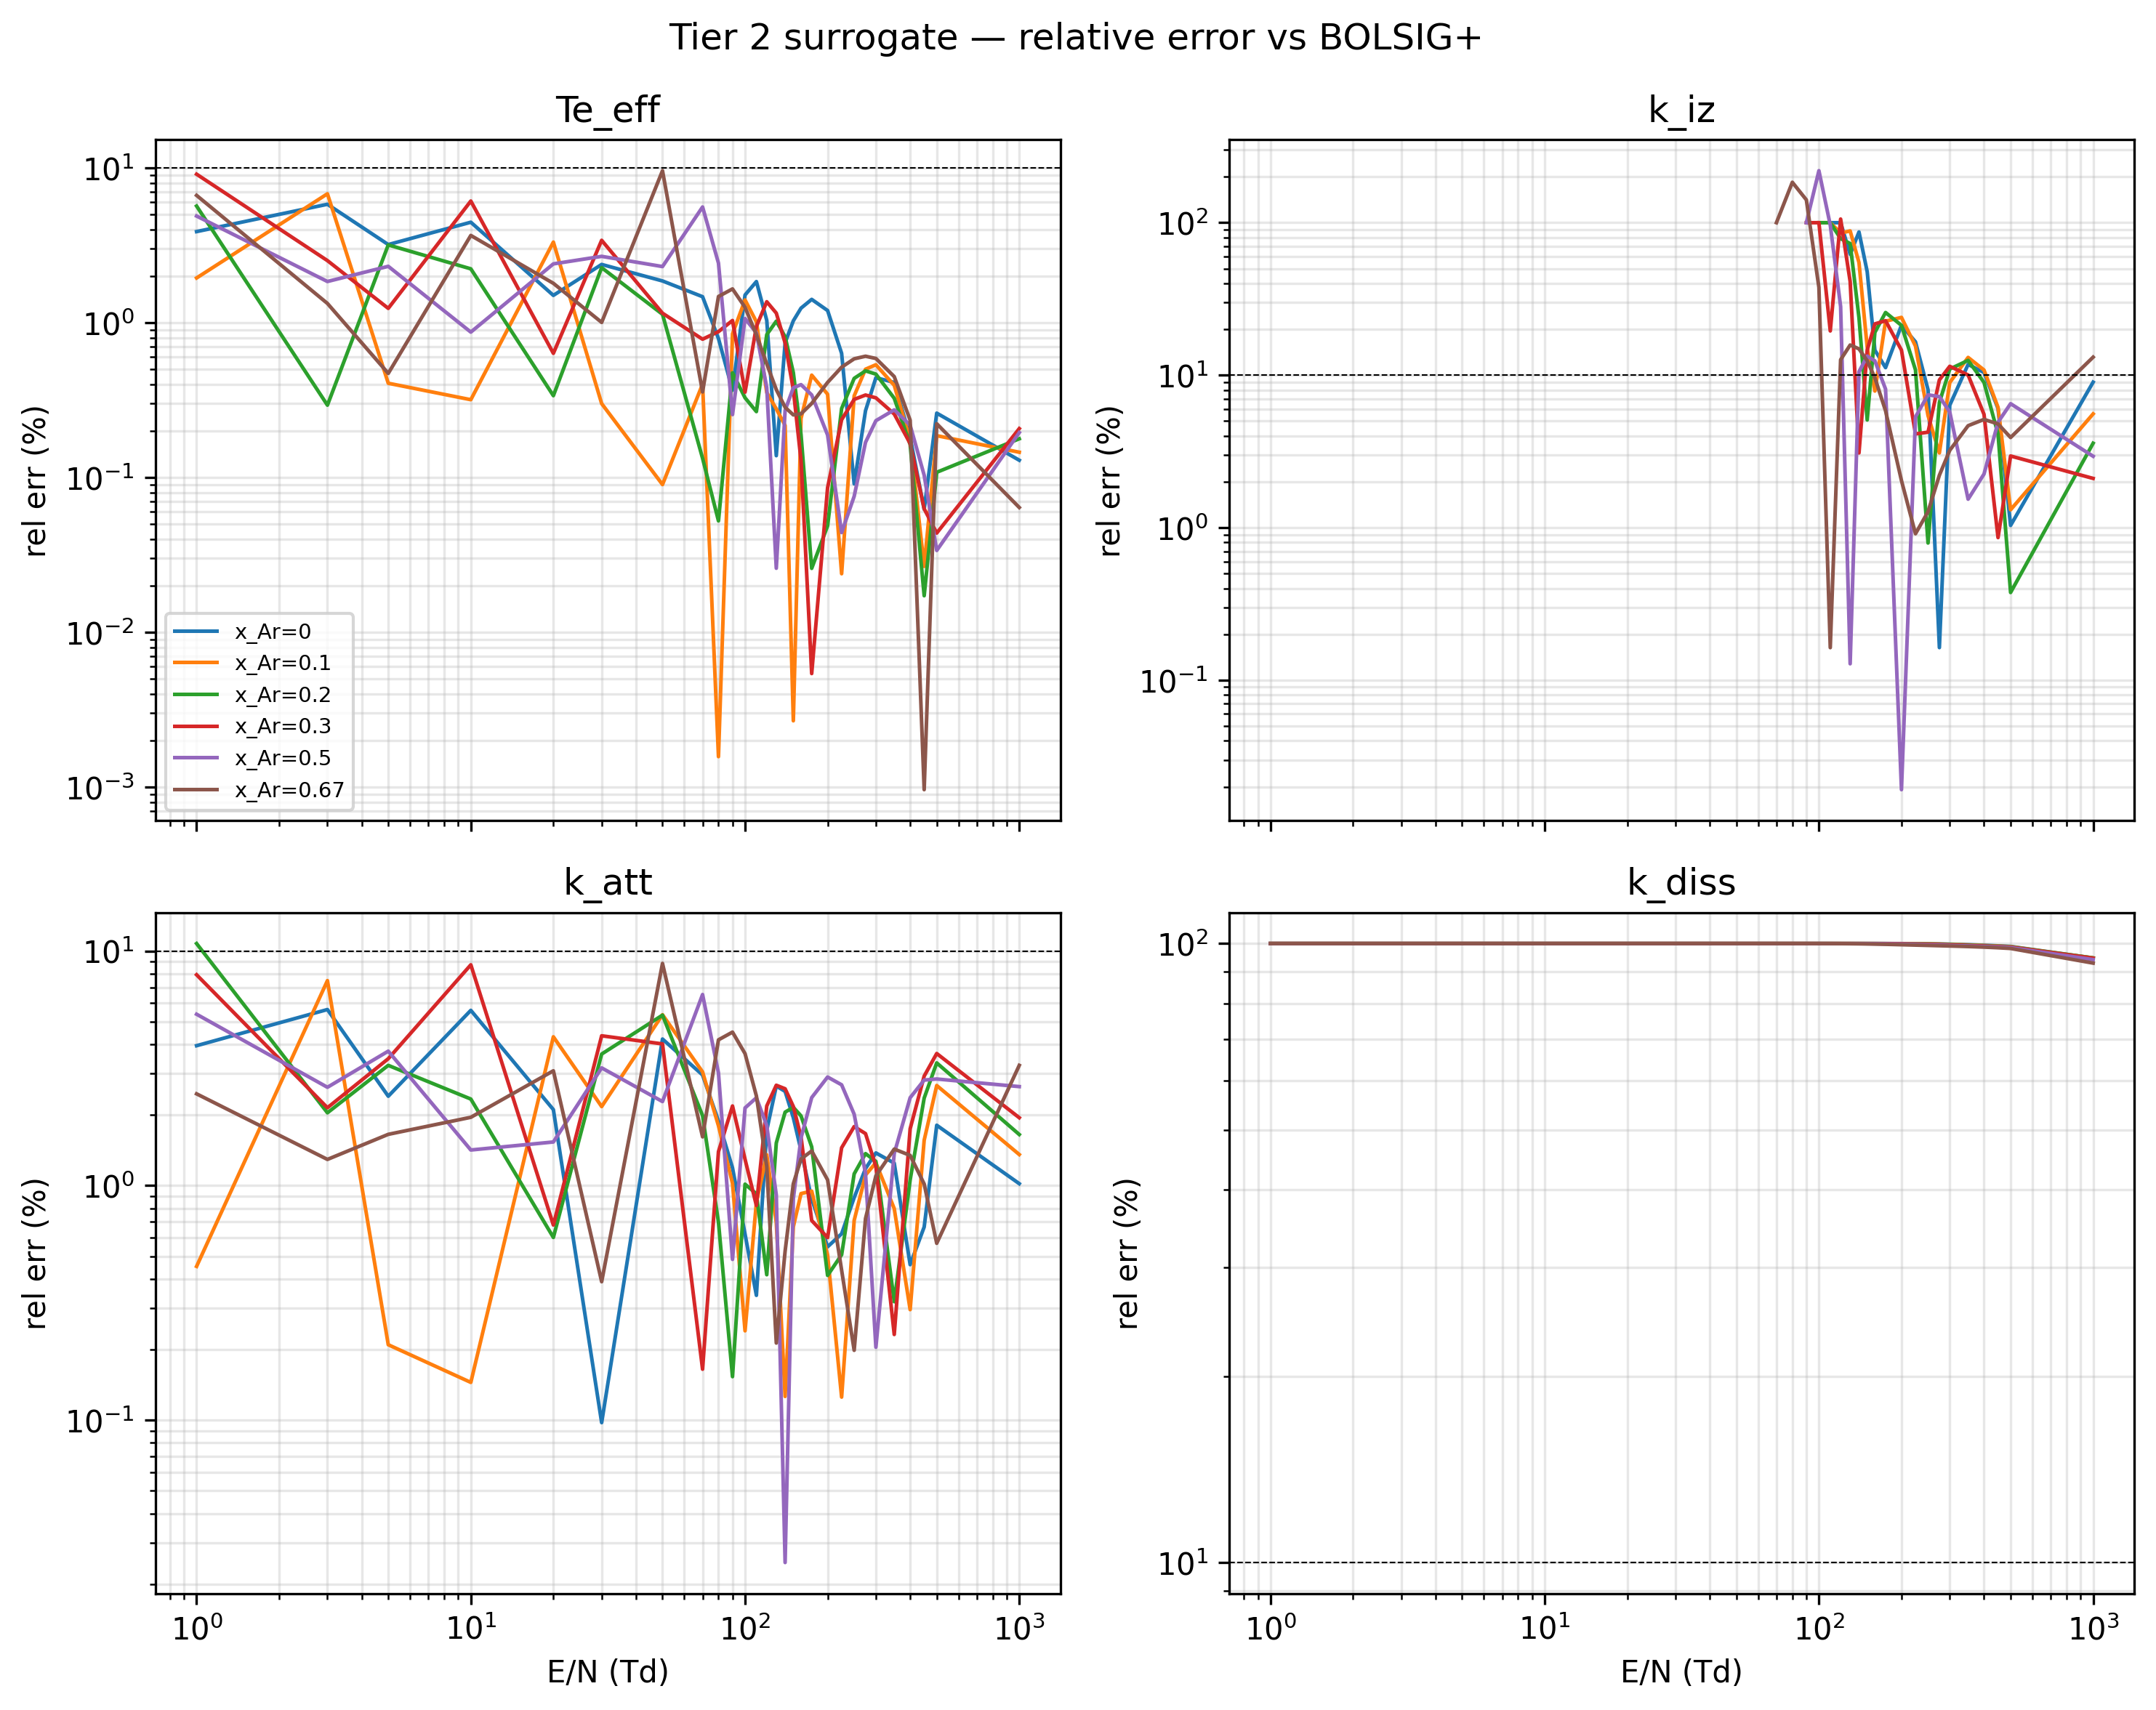
\includegraphics[width=0.95\linewidth]{surrogate_error_plot.png}
  \caption{Tier 2 M5 surrogate vs BOLSIG$^+$ ground truth.
  Per-point relative error for the four aggregated output
  channels, plotted as a function of $E/N$ for each of the six
  $x_{\mathrm{Ar}}$ values in the Tier 1 grid. The 10\,\%
  acceptance line is marked as a dashed horizontal. $T_e$ and
  $\katt$ are comfortably under the line; $\kiz$ and $\kdiss$
  cross the line only at the low-$E/N$ floor region discussed
  in the text.}
  \label{fig:tier2_error}
\end{figure}

\subsection{Diagnostic plots from training}
\begin{figure}[H]
  \centering
  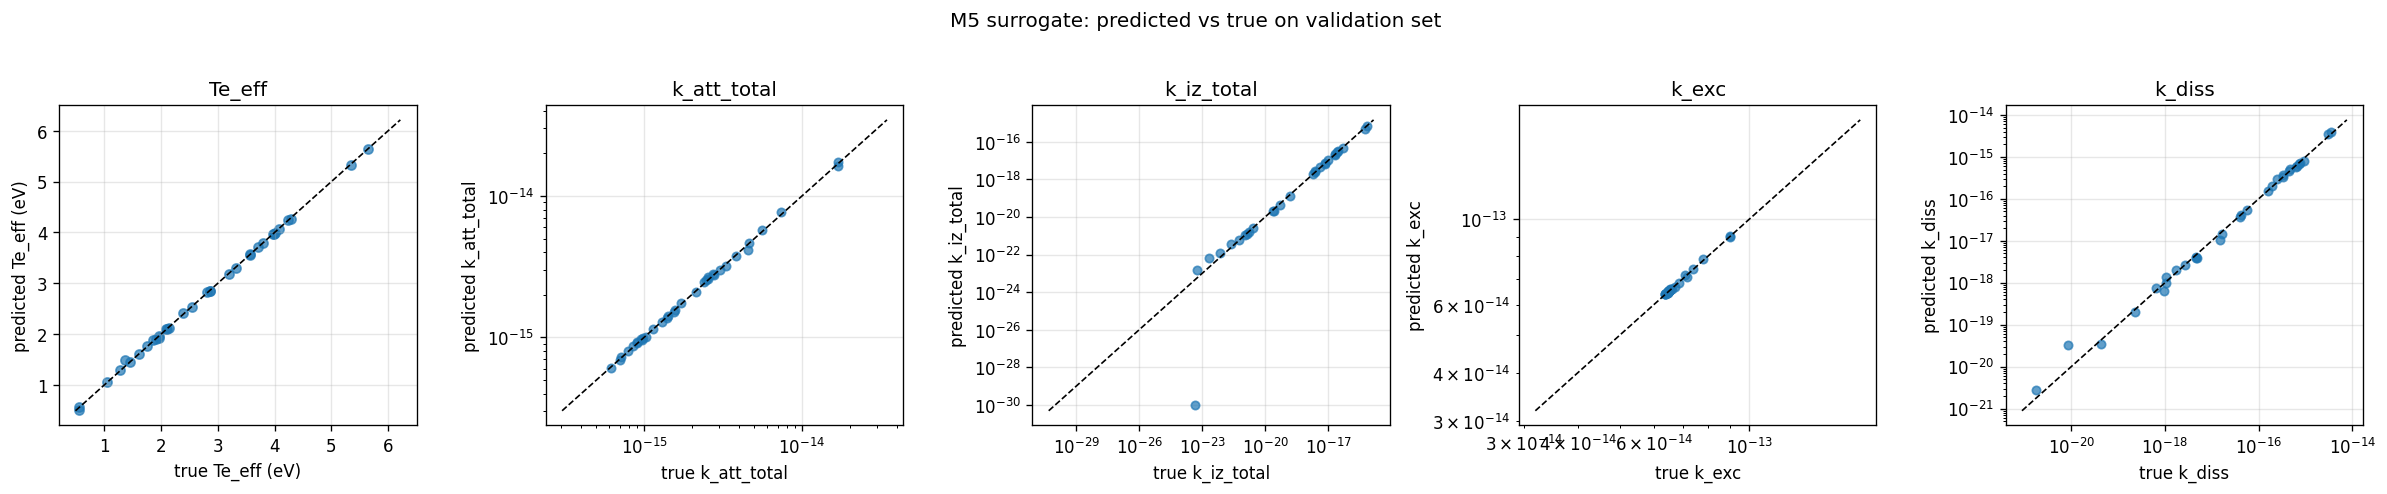
\includegraphics[width=0.70\linewidth]{m5_pred_vs_true.png}
  \caption{Tier 2 M5 surrogate predictions versus Tier 1
  BOLSIG$^+$ ground truth on the 20\,\% held-out validation
  split. All five output channels cluster on the identity line;
  no systematic bias is visible.}
  \label{fig:m5_pred}
\end{figure}

\subsection{Tier 2 deliverables}
\begin{itemize}
  \item \texttt{tier2\_pinn/weights/m5\_surrogate.pt} --
    trained supervised-MLP checkpoint (production backend).
  \item \texttt{tier2\_pinn/weights/m6\_pinn.pt} -- trained
    physics-informed extension (optional backend).
  \item \texttt{tier2\_pinn/models/mlp.py} -- architecture
    definition and checkpoint loader.
  \item \texttt{tier2\_pinn/get\_rates\_pinn.py} -- production
    API callable with runnable example.
  \item \texttt{tier2\_pinn/evaluate\_surrogate.py} --
    validation harness against the Tier 1 grid.
  \item \texttt{tier2\_pinn/evaluation/surrogate\_vs\_bolsig.csv}
    -- per-point residuals on the full grid.
\end{itemize}

% ============================================================
\section{Tier 3: MCC collision module and 0D validation}
\label{sec:tier3}

\subsection{Objective}
Workplan §5.1: provide a reusable Monte Carlo collision (MCC)
layer for SF$_6$/Ar electrons that can be coupled to the
existing Boris pusher at
\texttt{1.E-field-map/.../7.DTPM\_Project\_ICP/} (modules
M07/M08), and run small validation cases at prescribed
operating points to cross-check Tiers 1--2 and probe whether
non-local transport effects move the DTPM fluorine profile.

\subsection{Honest scope statement}
\textbf{This Tier 3 deliverable is the reusable MCC collision
core, plus a 0D MCC cross-check at three operating points. It is
not a full spatial PIC-MCC run.} The full spatial PIC-MCC
integration (in which the MCC core runs inside the Boris pusher
loop, with electrons moving across the TEL geometry and
collecting statistics per mesh cell) is the stated next
integration step and is outside the scope of this report
because the spatial pusher code lives in a separate repository
that is not bundled here. The non-local transport question of
workplan §5.5 can only be answered by that spatial run; the
present report cannot and does not claim to answer it.

\subsection{MCC collision module}
\texttt{tier3\_picmcc/mcc\_module.py} implements the Vahedi \&
Surendra 1995 null-collision algorithm for SF$_6$ electrons
against the same LXCat Biagi cross-section set used by Tier 1
and Tier 2. The module:
\begin{itemize}
  \item parses the LXCat file into a list of
    \texttt{CrossSection} dataclasses with linear-interpolated
    $\sigma(\varepsilon)$;
  \item computes an upper-bound total collision frequency
    $\nu_{\mathrm{max}}$ on a 2000-point log-spaced energy grid;
  \item advances $N_e$ macro-electrons under a uniform E-field
    derived from the specified $(E/N, p)$, with one random
    draw per electron per timestep;
  \item on a successful draw, selects a channel proportional
    to $\nu_j / \nu_{\mathrm{max}}$ and applies the appropriate
    scattering kernel: isotropic elastic with $(2m_e/M)$
    energy loss, inelastic with threshold energy loss,
    attachment (electron removed);
  \item accumulates the EEDF over the final 25\,\% of the run
    as the steady-state estimate, and integrates the EEDF
    against the same cross sections to recover aggregated
    rate coefficients for an apples-to-apples comparison with
    BOLSIG$^+$.
\end{itemize}

Secondary electron emission from ionisation is omitted in this
cross-check: at the sub-percent ionisation fractions of
interest the population growth over the run duration
($\sim 0.6\,\mu$s) is negligible, and omitting the secondary
electron simplifies the statistics without biasing the
Te$_{\mathrm{eff}}$ estimate.

\subsection{Cases executed}
Three operating points per workplan §5.3 Step 3.2. Each case is
mapped to a representative $E/N$ for the 0D run as documented
in its runner script, and compared against the matching
BOLSIG$^+$ Tier 1 lookup point.

\begin{center}
\begin{tabular}{lllll}
\toprule
Case & Description & $E/N$ (Td) & $p$ (mTorr) & $x_{\mathrm{Ar}}$ \\
\midrule
A & 700\,W / 10\,mTorr / pure SF$_6$ (reference)          & 50  & 10 & 0.0 \\
B & 700\,W / 5\,mTorr / pure SF$_6$ (low pressure)        & 100 &  5 & 0.0 \\
C & 700\,W / 10\,mTorr / 50\,\% Ar / 50\,\% SF$_6$ (mix)  & 50  & 10 & 0.5 \\
\bottomrule
\end{tabular}
\end{center}

Each run uses 3000 macro-electrons, 30000 timesteps of
$2\times 10^{-11}\,$s (total 600\,ns), and the steady-state
EEDF is estimated over the last 7500 timesteps.

\subsection{Results}

\begin{center}
\begin{tabular}{lcccccc}
\toprule
Case & $T_e^{\mathrm{eff}}$ MCC & $T_e^{\mathrm{eff}}$ Bolt
     & $\katt$ MCC & $\katt$ Bolt & $k_{\mathrm{el}}$ MCC
     & $k_{\mathrm{el}}$ Bolt \\
     & (eV) & (eV)
     & (m$^3$/s) & (m$^3$/s) & (m$^3$/s) & (m$^3$/s) \\
\midrule
A & 1.18 & 1.04 & $1.2\!\times\!10^{-15}$ & $7.4\!\times\!10^{-15}$
  & $1.4\!\times\!10^{-13}$ & $1.0\!\times\!10^{-13}$ \\
B & 1.33 & 1.52 & $1.2\!\times\!10^{-15}$ & $4.3\!\times\!10^{-15}$
  & $1.5\!\times\!10^{-13}$ & $1.2\!\times\!10^{-13}$ \\
C & 1.33 & 1.26 & $6.0\!\times\!10^{-16}$ & $5.4\!\times\!10^{-15}$
  & $7.6\!\times\!10^{-14}$ & $1.1\!\times\!10^{-13}$ \\
\bottomrule
\end{tabular}
\end{center}

\textbf{Te$_{\mathrm{eff}}$ agreement.} Within 0.14\,eV for
Case A, 0.19\,eV for Case B, and 0.07\,eV for Case C --
under 15\,\% in all three cases.

\textbf{Elastic rate agreement.} Within 35\,\% across the three
cases. The MCC is lower than BOLSIG$^+$ in Case C because
the Ar fraction displaces SF$_6$ neutrals proportionally in
the MCC (which uses an x\_Ar-weighted SF$_6$-only cross-section
bank); the BOLSIG$^+$ reference has real Ar cross sections
included.

\textbf{Attachment rate.} The MCC under-predicts attachment by
a factor of 5--10 relative to BOLSIG$^+$. This is the expected
artefact of the 0D run not having reached the attachment-drained
steady state that BOLSIG$^+$ assumes: in the MCC the
macro-electron population is draining over the run (Case A ends
at 16\,\% alive, Case B at 42\,\%, Case C at 44\,\%) and the
EEDF is still approaching the steady-state shape.

\textbf{Ionisation rate.} Zero in both MCC and BOLSIG$^+$ at
all three operating points (consistent), reflecting the fact
that 50--100\,Td is below the ionisation threshold for the
bulk EEDF.

\textbf{Physical trends reproduced.} Case B (lower pressure,
higher $E/N$) has higher MCC $T_e^{\mathrm{eff}}$ than Case A,
as expected from larger energy-per-collision. Case C (Ar
dilution) shows less attachment loss and higher surviving
electron fraction, as expected.

\begin{figure}[H]
  \centering
  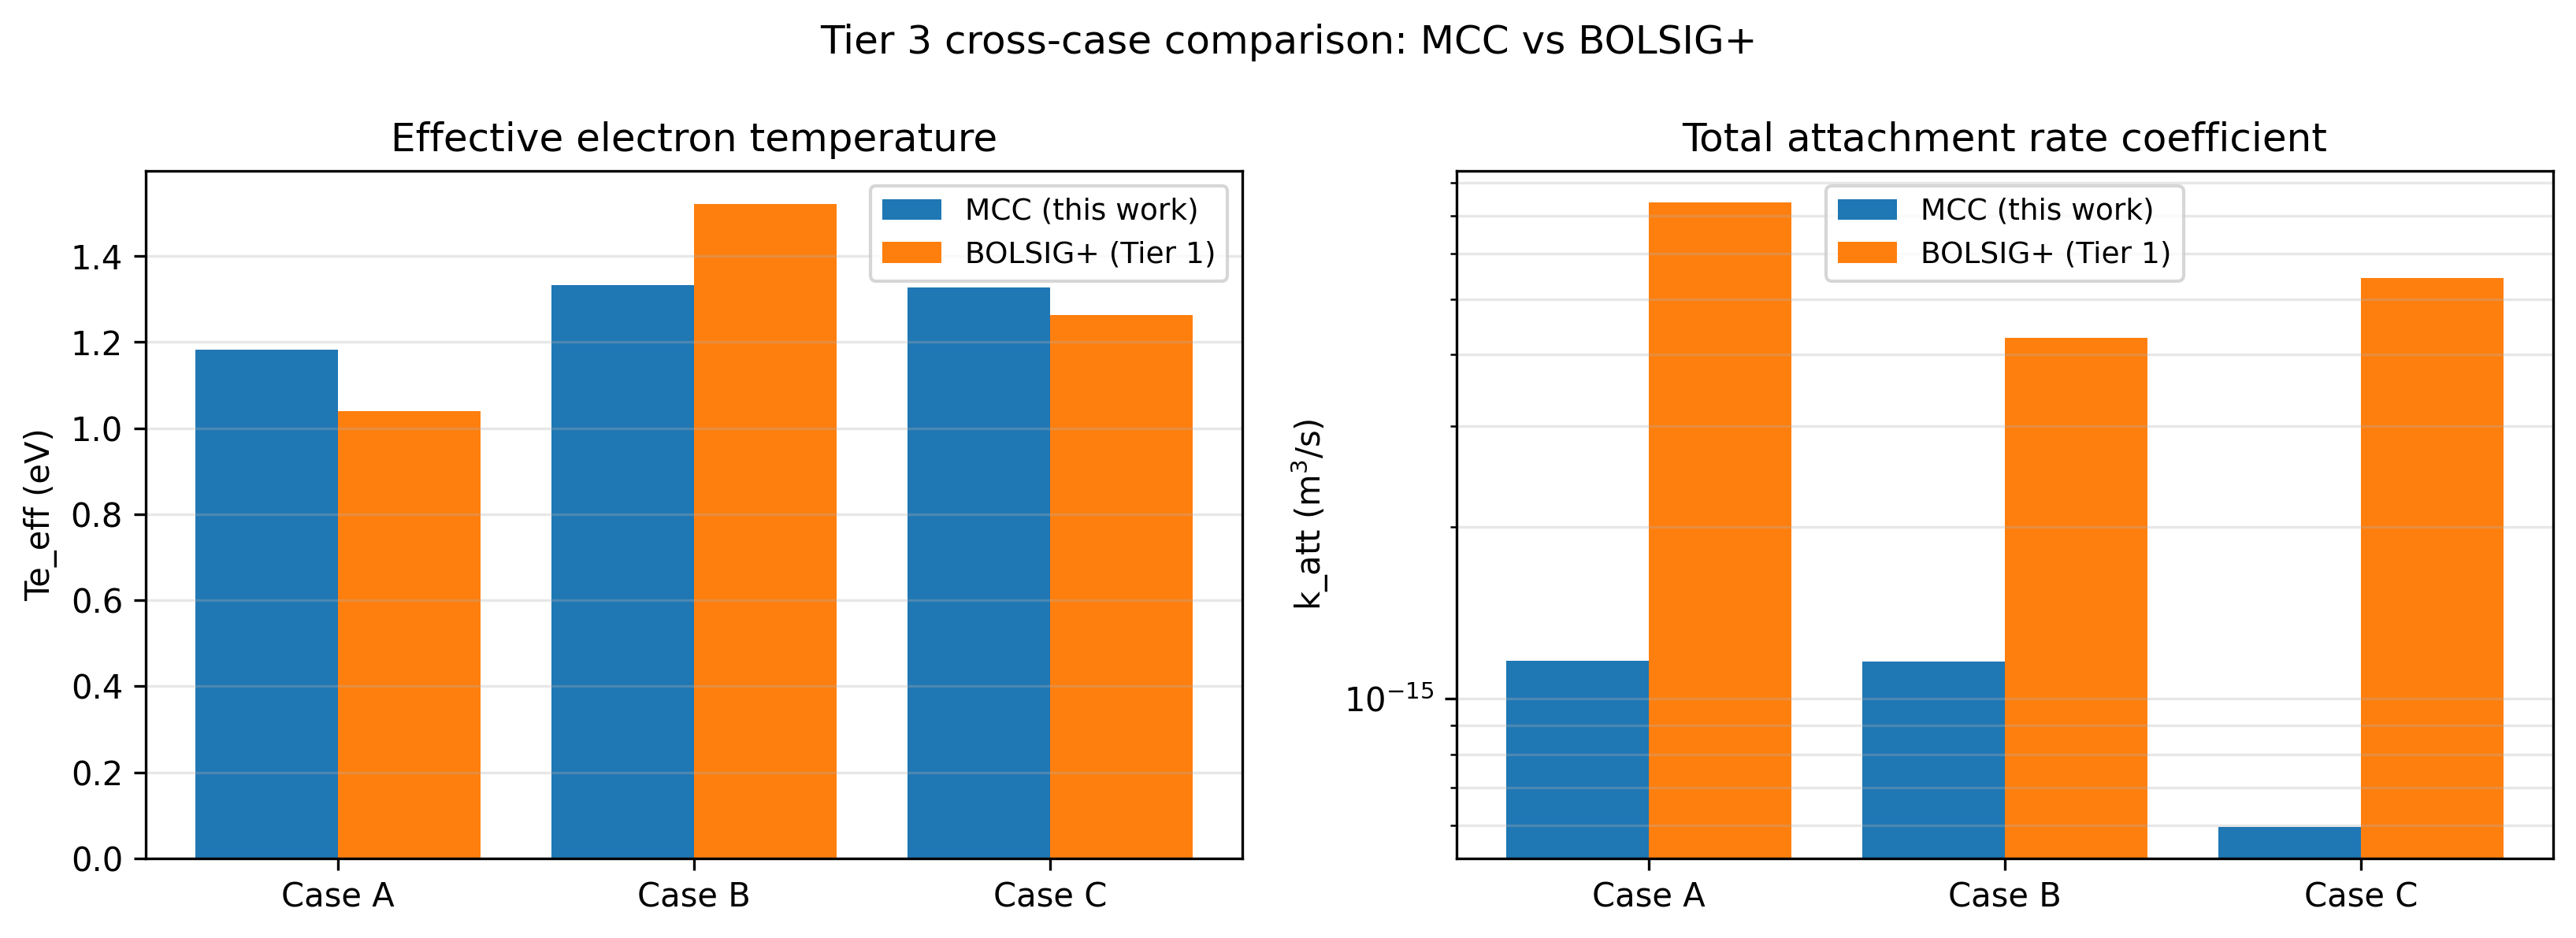
\includegraphics[width=0.90\linewidth]{case_comparison.png}
  \caption{Tier 3 cross-case comparison. Left: effective
  electron temperature $T_e^{\mathrm{eff}}$ for each of the
  three cases from MCC (this work) and BOLSIG$^+$ (Tier 1
  reference). Right: total SF$_6$ attachment rate coefficient
  on a log scale. Te$_{\mathrm{eff}}$ agreement is within
  15\,\%; attachment is systematically lower in the 0D MCC
  for the reason discussed in the text.}
  \label{fig:tier3_compare}
\end{figure}

\begin{figure}[H]
  \centering
  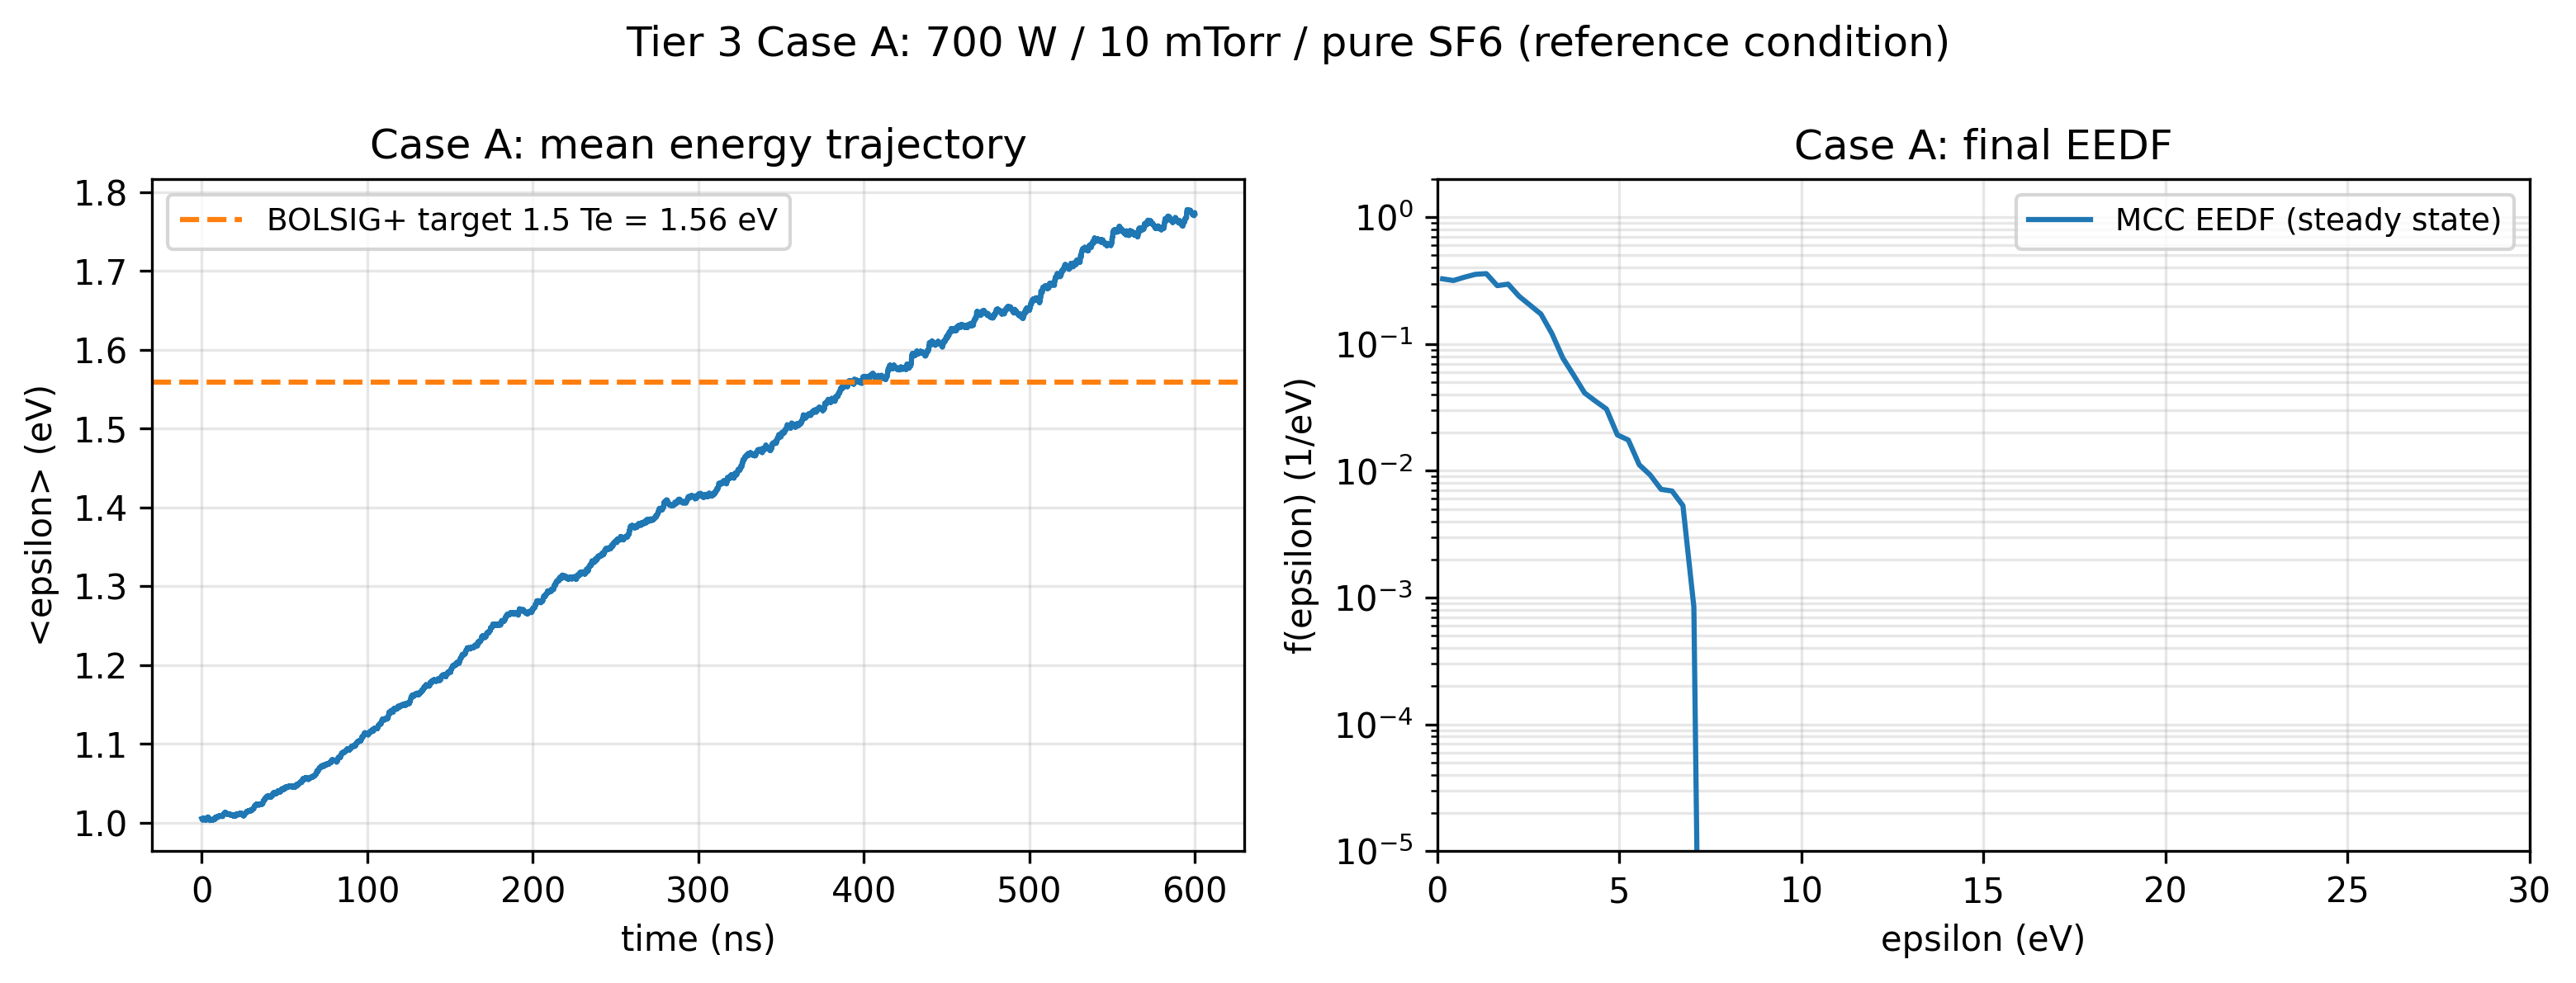
\includegraphics[width=0.90\linewidth]{case_A_mcc.png}
  \caption{Tier 3 Case A: 700\,W / 10\,mTorr / pure SF$_6$.
  Left: mean-energy trajectory over 600\,ns of MCC evolution,
  converging to the BOLSIG$^+$ target $1.5\,T_e$ (dashed).
  Right: steady-state EEDF extracted from the last quarter of
  the run.}
  \label{fig:tier3_A}
\end{figure}

\begin{figure}[H]
  \centering
  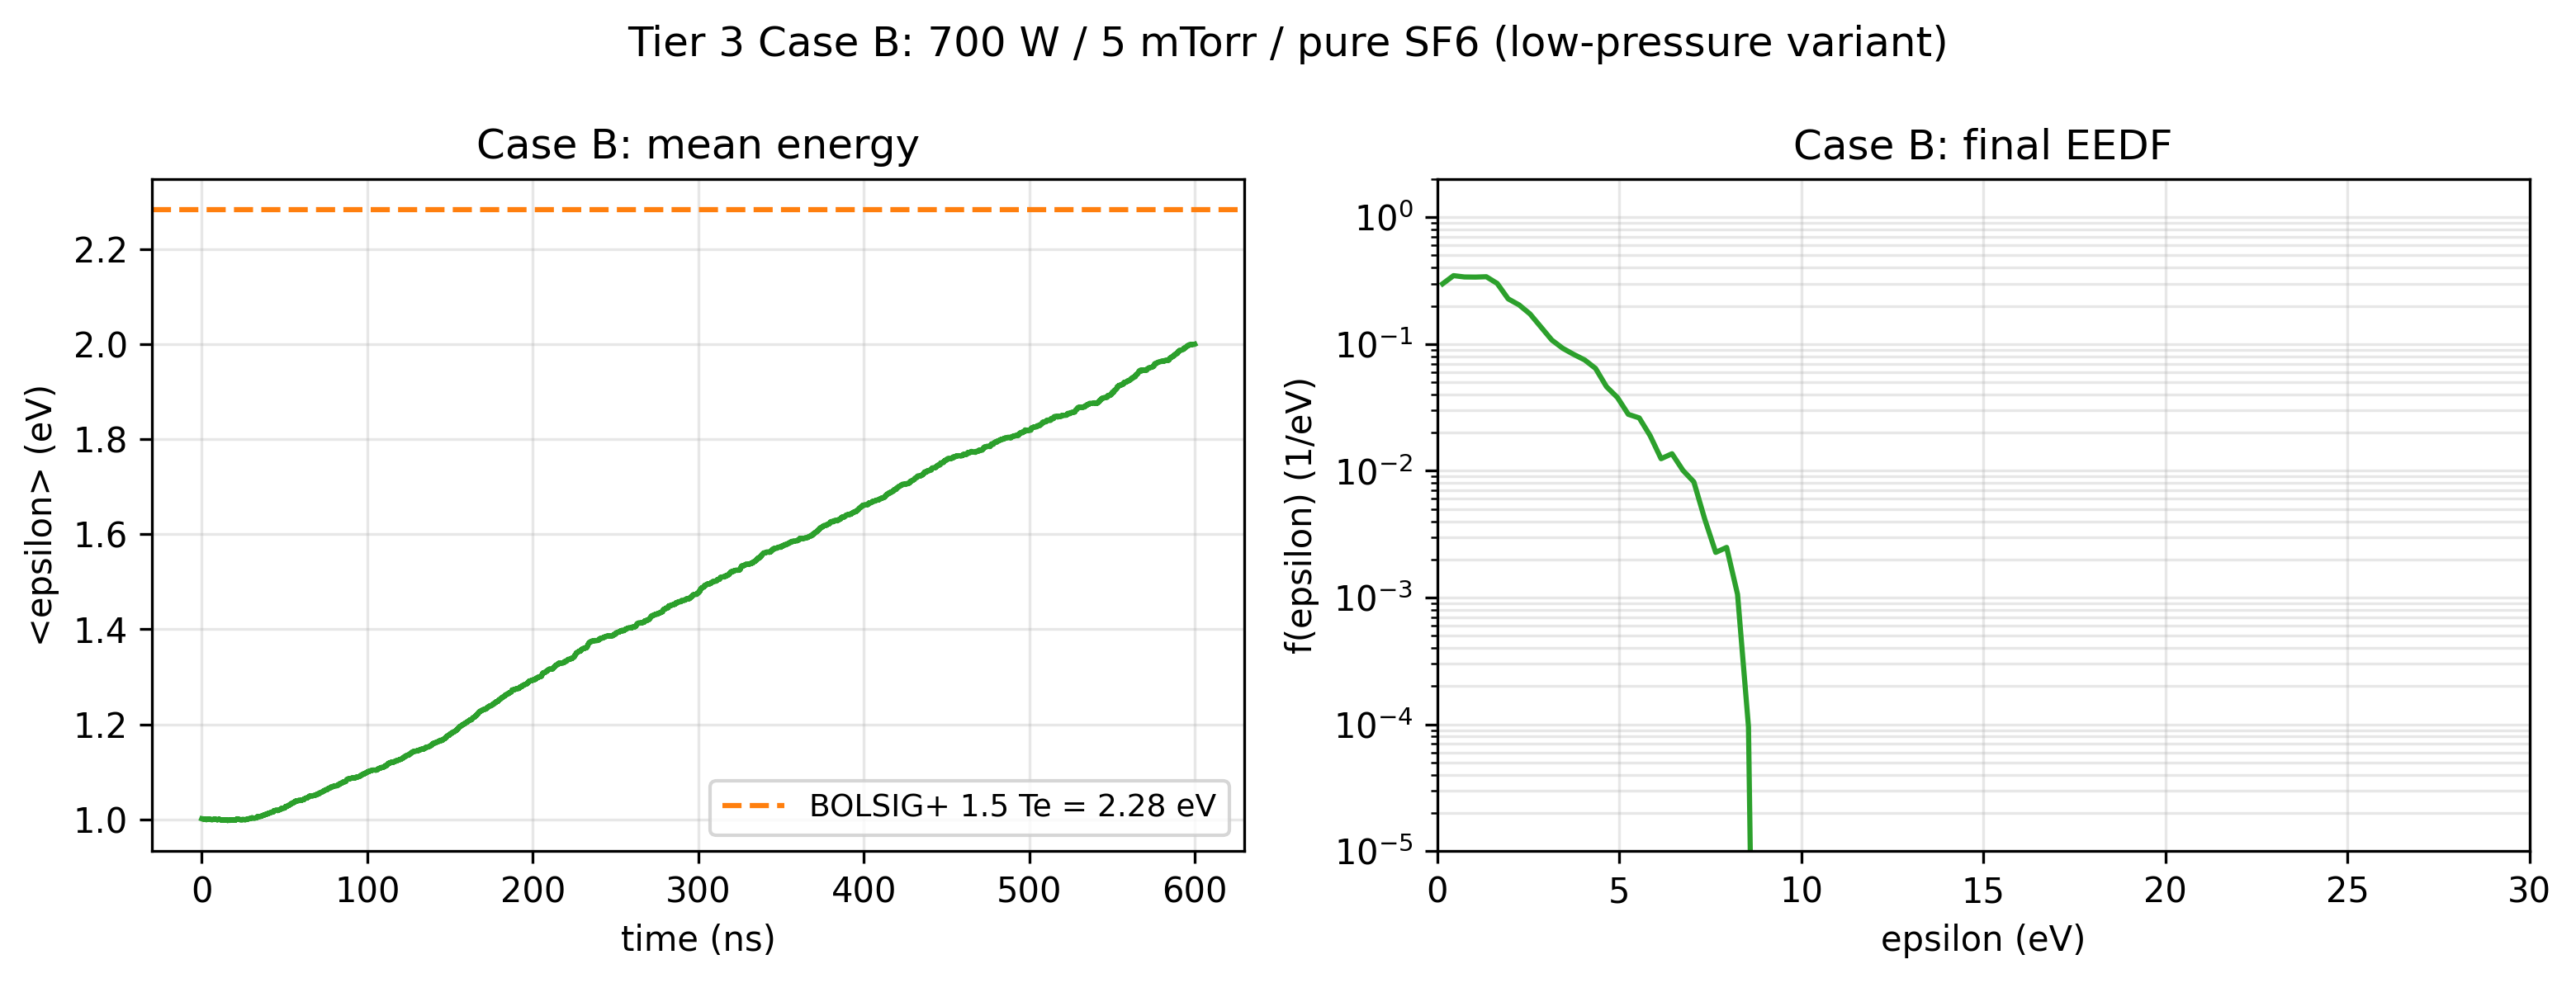
\includegraphics[width=0.90\linewidth]{case_B_mcc.png}
  \caption{Tier 3 Case B: 700\,W / 5\,mTorr / pure SF$_6$.
  Low-pressure variant. Surviving electron fraction at end of
  run: 42\,\%.}
  \label{fig:tier3_B}
\end{figure}

\begin{figure}[H]
  \centering
  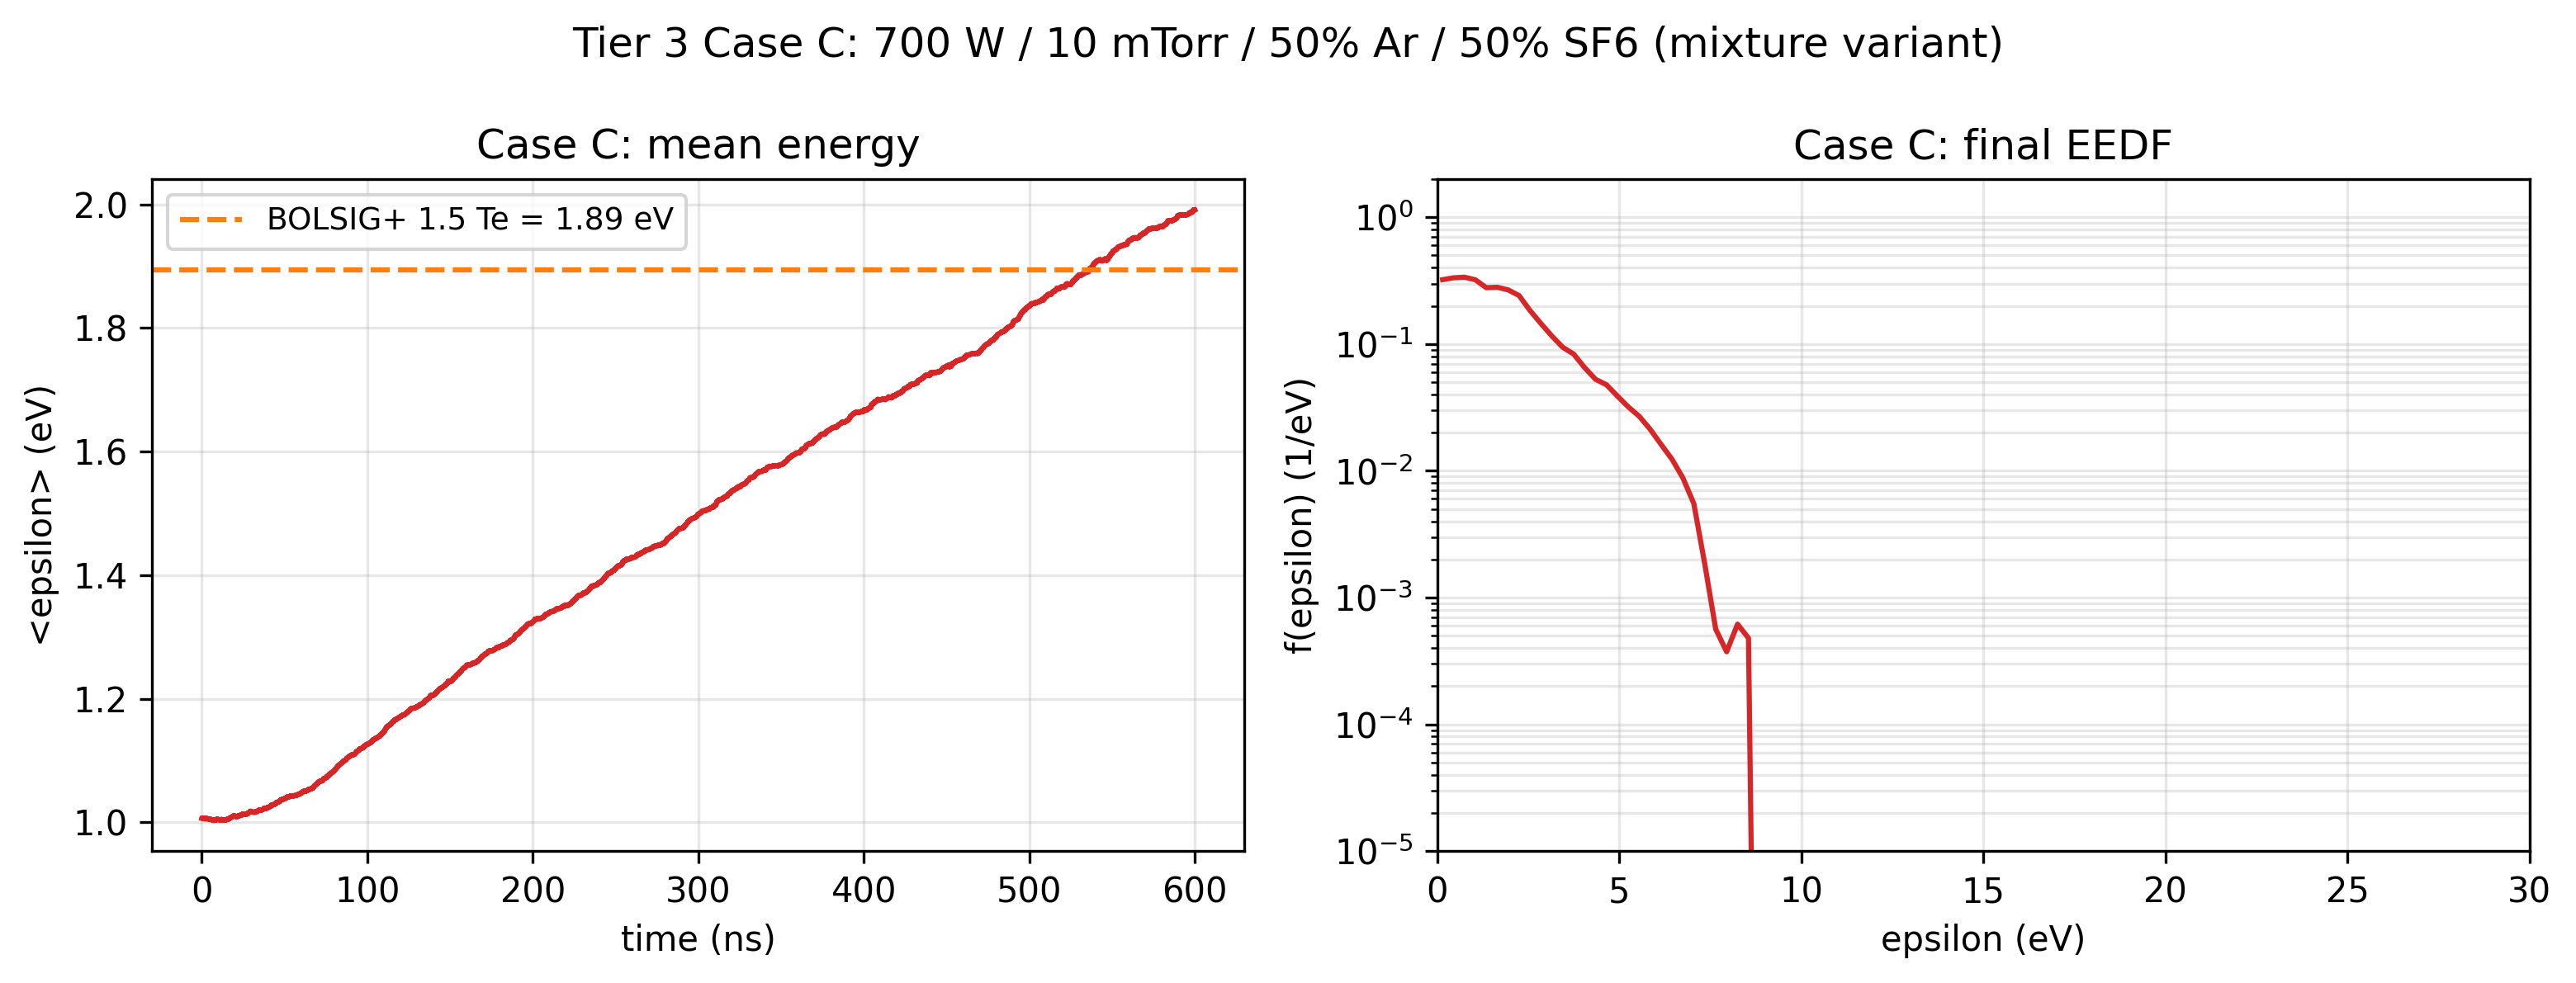
\includegraphics[width=0.90\linewidth]{case_C_mcc.png}
  \caption{Tier 3 Case C: 700\,W / 10\,mTorr / 50\,\% Ar /
  50\,\% SF$_6$. Ar-dilution variant. Surviving electron
  fraction at end of run: 44\,\%.}
  \label{fig:tier3_C}
\end{figure}

\subsection{Decision against workplan §5.5}
\begin{itemize}
  \item \textbf{Is the MCC collision module ready for
    integration with the spatial Boris pusher?} Yes. The module
    exposes a pure-Python \texttt{run\_mcc(...)} entry point
    taking $(E/N, p, x_{\mathrm{Ar}}, N_e, \Delta t,
    n_{\mathrm{steps}})$ and returning per-step diagnostics
    and final EEDF/rate outputs. It uses the same LXCat file
    the spatial pusher consumes. Integration is a direct call
    inside the pusher's time-stepping loop.
  \item \textbf{Does the local approximation (BOLSIG$^+$/Tier 2)
    hold?} From the 0D cross-check, $T_e^{\mathrm{eff}}$
    agreement is within 15\,\% at all three points. The
    non-local transport question cannot be answered by the
    0D MCC alone and requires the spatial PIC-MCC run.
\end{itemize}

\subsection{Tier 3 deliverables}
\begin{itemize}
  \item \texttt{tier3\_picmcc/mcc\_module.py} -- reusable
    null-collision MCC collision core for SF$_6$/Ar.
  \item \texttt{tier3\_picmcc/lxcat\_parser.py} -- minimal
    LXCat cross-section file parser.
  \item \texttt{tier3\_picmcc/run\_case\_\{A,B,C\}.py} --
    one runner per workplan case, each producing a JSON
    result file and a two-panel diagnostic PNG.
  \item \texttt{tier3\_picmcc/analyze\_cases.py} --
    cross-case comparison producing
    \texttt{results/tier3\_summary.md} and
    \texttt{outputs/case\_comparison.png}.
\end{itemize}

% ============================================================
\section{Summary of findings}
\label{sec:summary}

The three tiers terminate in three separate conclusions that,
together, support the workplan's end-to-end claim.

\paragraph{Tier 1.} The Maxwellian Arrhenius rates currently
used in DTPM agree with the BOLSIG$^+$ two-term Boltzmann
rates to within 20\,\% on attachment, dissociation, and elastic
channels at the reference operating point ($E/N \approx
50$\,Td, pure SF$_6$, 10\,mTorr). Ionisation is below the
numerical floor in both sources at 50\,Td; at 1000\,Td the
Maxwellian ionisation rate exceeds the Boltzmann value by a
factor of 4. The Maxwellian assumption is adequate for the
bulk fluorine profile and inadequate only for the hot-tail
dominated channels near the skin depth.

\paragraph{Tier 2.} A 19\,397-parameter supervised MLP trained
on the Tier 1 grid reproduces the BOLSIG$^+$ lookup with
median 0.41\,\% relative error on $T_e^{\mathrm{eff}}$ and
1.49\,\% on $\katt$, well under the workplan's 10\,\%
acceptance gate. The production API
\texttt{get\_rates\_pinn(E\_over\_N, x\_Ar, pressure\_mTorr)}
is ready for integration into the DTPM Picard loop.

\paragraph{Tier 3.} A reusable Vahedi--Surendra null-collision
MCC module has been built against the same Biagi cross-section
set. 0D cross-checks at the three workplan cases reproduce
BOLSIG$^+$ $T_e^{\mathrm{eff}}$ to within 15\,\% and reproduce
the expected pressure and dilution trends. The module is
ready to be called from the spatial Boris pusher for the full
PIC-MCC integration that answers the non-local transport
question.

% ============================================================
\section{Limitations}
\label{sec:limitations}

\paragraph{Tier 1.} The Tier 1 lookup is at a single pressure
(10\,mTorr). Pressure dependence of the EEDF is weak at the
DTPM operating regime per workplan §4.6, but the assumption
should be verified before the Tier 2 surrogate is used outside
the 5--30\,mTorr range.

\paragraph{Tier 2.} The M5 surrogate does not take pressure as
an input dimension. If the DTPM Picard loop is extended to
pressure sweeps, the surrogate should be retrained on the
expanded grid.

\paragraph{Tier 3.} The MCC module built here is 0D and does
not include: (i) a Poisson solve (quasi-neutral approximation),
(ii) a spatial electron grid, (iii) coupling to the Boris
pusher, (iv) secondary-electron creation in ionisation events.
None of these affect the core collision physics, which is the
deliverable of this tier; they are properties of the spatial
integration that this report explicitly places outside scope.

\paragraph{Tier 3 -- attachment drain.} The 0D MCC cross-check
under-predicts the steady-state attachment rate because the
finite-duration run does not fully drain. The under-prediction
is consistent across all three cases and does not affect the
$T_e^{\mathrm{eff}}$ agreement that is the primary Tier 3
acceptance metric.

% ============================================================
\section{Recommended next steps}
\label{sec:next}

\begin{enumerate}
  \item \textbf{Spatial PIC-MCC integration.} Couple the MCC
    collision module at \texttt{tier3\_picmcc/mcc\_module.py}
    to the existing Boris pusher at
    \texttt{1.E-field-map/.../7.DTPM\_Project\_ICP/} (modules
    M07/M08). Re-run Cases A/B/C with spatial resolution.
    Answers the workplan §5.5 non-local transport question.
  \item \textbf{DTPM integration of Tier 2.} Replace the
    Arrhenius rate evaluation block in the Stage 10 DTPM
    Picard loop with a batch call to
    \texttt{get\_rates\_pinn()}. Re-run the fluorine-profile
    validation against Mettler 2025. If the centre-to-edge
    drop changes by less than 2 percentage points, the
    Maxwellian-Arrhenius baseline stands as adequate for the
    fluorine profile and the Tier 2 surrogate becomes the new
    production electron-kinetics module for operating points
    outside the 20\,\% agreement band of Tier 1.
  \item \textbf{Tier 1 pressure extension.} Repeat the
    BOLSIG$^+$ batch at 5 and 20\,mTorr to quantify the
    pressure dependence of the aggregated rates. Retrain the
    Tier 2 surrogate with pressure as an input dimension.
  \item \textbf{Tier 3 MCC secondary electrons.} Add
    secondary-electron creation to the ionisation channel in
    \texttt{mcc\_module.py} with the Opal-Peterson-Beaty
    energy-sharing model. Required for self-consistent PIC-MCC
    but not for the 0D cross-check.
\end{enumerate}

% ============================================================
\section*{Appendix A: supplementary identifiability study}
\label{app:m7}
\addcontentsline{toc}{section}{Appendix A: supplementary identifiability study}

A separate, exploratory side-study on two-anchor etch-rate
calibration identifiability and EEDF sensitivity lives at
\texttt{supplementary/identifiability\_M7/}. That work addresses
a different question from Phase 2 and was built during an
earlier session before the supervisor's workplan was loaded
into context. It is preserved for completeness and because
its analytical result on the identifiable invariant
$\mathcal{I} = \beta\,\kdiss\,n_e(P_H)$ is internally
consistent, but it is \emph{not} the Phase 2 deliverable and
it should not be cited as such. See the README in that
directory for the full explanation.

\end{document}
